


% Header, overrides base

    % Make sure that the sphinx doc style knows who it inherits from.
    \def\sphinxdocclass{article}

    % Declare the document class
    \documentclass[letterpaper,10pt,english]{/usr/local/lib/python2.7/dist-packages/Sphinx-1.2b1-py2.7.egg/sphinx/texinputs/sphinxhowto}

    % Imports
    \usepackage[utf8]{inputenc}
    \DeclareUnicodeCharacter{00A0}{\\nobreakspace}
    \usepackage[T1]{fontenc}
    \usepackage{babel}
    \usepackage{times}
    \usepackage{import}
    \usepackage[Bjarne]{/usr/local/lib/python2.7/dist-packages/Sphinx-1.2b1-py2.7.egg/sphinx/texinputs/fncychap}
    \usepackage{longtable}
    \usepackage{/usr/local/lib/python2.7/dist-packages/Sphinx-1.2b1-py2.7.egg/sphinx/texinputs/sphinx}
    \usepackage{multirow}

    \usepackage{amsmath}
    \usepackage{amssymb}
    \usepackage{ucs}
    \usepackage{enumerate}

    % Used to make the Input/Output rules follow around the contents.
    \usepackage{needspace}

    % Pygments requirements
    \usepackage{fancyvrb}
    \usepackage{color}
    % ansi colors additions
    \definecolor{darkgreen}{rgb}{.12,.54,.11}
    \definecolor{lightgray}{gray}{.95}
    \definecolor{brown}{rgb}{0.54,0.27,0.07}
    \definecolor{purple}{rgb}{0.5,0.0,0.5}
    \definecolor{darkgray}{gray}{0.25}
    \definecolor{lightred}{rgb}{1.0,0.39,0.28}
    \definecolor{lightgreen}{rgb}{0.48,0.99,0.0}
    \definecolor{lightblue}{rgb}{0.53,0.81,0.92}
    \definecolor{lightpurple}{rgb}{0.87,0.63,0.87}
    \definecolor{lightcyan}{rgb}{0.5,1.0,0.83}

    % Needed to box output/input
    \usepackage{tikz}
        \usetikzlibrary{calc,arrows,shadows}
    \usepackage[framemethod=tikz]{mdframed}

    \usepackage{alltt}

    % Used to load and display graphics
    \usepackage{graphicx}
    \graphicspath{ {figs/} }
    \usepackage[Export]{adjustbox} % To resize


    % For formatting output while also word wrapping.
    \usepackage{listings}
    \lstset{breaklines=true}
    \lstset{basicstyle=\small\ttfamily}
    \def\smaller{\fontsize{9.5pt}{9.5pt}\selectfont}

    %Pygments definitions
    
\makeatletter
\def\PY@reset{\let\PY@it=\relax \let\PY@bf=\relax%
    \let\PY@ul=\relax \let\PY@tc=\relax%
    \let\PY@bc=\relax \let\PY@ff=\relax}
\def\PY@tok#1{\csname PY@tok@#1\endcsname}
\def\PY@toks#1+{\ifx\relax#1\empty\else%
    \PY@tok{#1}\expandafter\PY@toks\fi}
\def\PY@do#1{\PY@bc{\PY@tc{\PY@ul{%
    \PY@it{\PY@bf{\PY@ff{#1}}}}}}}
\def\PY#1#2{\PY@reset\PY@toks#1+\relax+\PY@do{#2}}

\expandafter\def\csname PY@tok@gd\endcsname{\def\PY@tc##1{\textcolor[rgb]{0.63,0.00,0.00}{##1}}}
\expandafter\def\csname PY@tok@gu\endcsname{\let\PY@bf=\textbf\def\PY@tc##1{\textcolor[rgb]{0.50,0.00,0.50}{##1}}}
\expandafter\def\csname PY@tok@gt\endcsname{\def\PY@tc##1{\textcolor[rgb]{0.00,0.27,0.87}{##1}}}
\expandafter\def\csname PY@tok@gs\endcsname{\let\PY@bf=\textbf}
\expandafter\def\csname PY@tok@gr\endcsname{\def\PY@tc##1{\textcolor[rgb]{1.00,0.00,0.00}{##1}}}
\expandafter\def\csname PY@tok@cm\endcsname{\let\PY@it=\textit\def\PY@tc##1{\textcolor[rgb]{0.25,0.50,0.50}{##1}}}
\expandafter\def\csname PY@tok@vg\endcsname{\def\PY@tc##1{\textcolor[rgb]{0.10,0.09,0.49}{##1}}}
\expandafter\def\csname PY@tok@m\endcsname{\def\PY@tc##1{\textcolor[rgb]{0.40,0.40,0.40}{##1}}}
\expandafter\def\csname PY@tok@mh\endcsname{\def\PY@tc##1{\textcolor[rgb]{0.40,0.40,0.40}{##1}}}
\expandafter\def\csname PY@tok@go\endcsname{\def\PY@tc##1{\textcolor[rgb]{0.53,0.53,0.53}{##1}}}
\expandafter\def\csname PY@tok@ge\endcsname{\let\PY@it=\textit}
\expandafter\def\csname PY@tok@vc\endcsname{\def\PY@tc##1{\textcolor[rgb]{0.10,0.09,0.49}{##1}}}
\expandafter\def\csname PY@tok@il\endcsname{\def\PY@tc##1{\textcolor[rgb]{0.40,0.40,0.40}{##1}}}
\expandafter\def\csname PY@tok@cs\endcsname{\let\PY@it=\textit\def\PY@tc##1{\textcolor[rgb]{0.25,0.50,0.50}{##1}}}
\expandafter\def\csname PY@tok@cp\endcsname{\def\PY@tc##1{\textcolor[rgb]{0.74,0.48,0.00}{##1}}}
\expandafter\def\csname PY@tok@gi\endcsname{\def\PY@tc##1{\textcolor[rgb]{0.00,0.63,0.00}{##1}}}
\expandafter\def\csname PY@tok@gh\endcsname{\let\PY@bf=\textbf\def\PY@tc##1{\textcolor[rgb]{0.00,0.00,0.50}{##1}}}
\expandafter\def\csname PY@tok@ni\endcsname{\let\PY@bf=\textbf\def\PY@tc##1{\textcolor[rgb]{0.60,0.60,0.60}{##1}}}
\expandafter\def\csname PY@tok@nl\endcsname{\def\PY@tc##1{\textcolor[rgb]{0.63,0.63,0.00}{##1}}}
\expandafter\def\csname PY@tok@nn\endcsname{\let\PY@bf=\textbf\def\PY@tc##1{\textcolor[rgb]{0.00,0.00,1.00}{##1}}}
\expandafter\def\csname PY@tok@no\endcsname{\def\PY@tc##1{\textcolor[rgb]{0.53,0.00,0.00}{##1}}}
\expandafter\def\csname PY@tok@na\endcsname{\def\PY@tc##1{\textcolor[rgb]{0.49,0.56,0.16}{##1}}}
\expandafter\def\csname PY@tok@nb\endcsname{\def\PY@tc##1{\textcolor[rgb]{0.00,0.50,0.00}{##1}}}
\expandafter\def\csname PY@tok@nc\endcsname{\let\PY@bf=\textbf\def\PY@tc##1{\textcolor[rgb]{0.00,0.00,1.00}{##1}}}
\expandafter\def\csname PY@tok@nd\endcsname{\def\PY@tc##1{\textcolor[rgb]{0.67,0.13,1.00}{##1}}}
\expandafter\def\csname PY@tok@ne\endcsname{\let\PY@bf=\textbf\def\PY@tc##1{\textcolor[rgb]{0.82,0.25,0.23}{##1}}}
\expandafter\def\csname PY@tok@nf\endcsname{\def\PY@tc##1{\textcolor[rgb]{0.00,0.00,1.00}{##1}}}
\expandafter\def\csname PY@tok@si\endcsname{\let\PY@bf=\textbf\def\PY@tc##1{\textcolor[rgb]{0.73,0.40,0.53}{##1}}}
\expandafter\def\csname PY@tok@s2\endcsname{\def\PY@tc##1{\textcolor[rgb]{0.73,0.13,0.13}{##1}}}
\expandafter\def\csname PY@tok@vi\endcsname{\def\PY@tc##1{\textcolor[rgb]{0.10,0.09,0.49}{##1}}}
\expandafter\def\csname PY@tok@nt\endcsname{\let\PY@bf=\textbf\def\PY@tc##1{\textcolor[rgb]{0.00,0.50,0.00}{##1}}}
\expandafter\def\csname PY@tok@nv\endcsname{\def\PY@tc##1{\textcolor[rgb]{0.10,0.09,0.49}{##1}}}
\expandafter\def\csname PY@tok@s1\endcsname{\def\PY@tc##1{\textcolor[rgb]{0.73,0.13,0.13}{##1}}}
\expandafter\def\csname PY@tok@sh\endcsname{\def\PY@tc##1{\textcolor[rgb]{0.73,0.13,0.13}{##1}}}
\expandafter\def\csname PY@tok@sc\endcsname{\def\PY@tc##1{\textcolor[rgb]{0.73,0.13,0.13}{##1}}}
\expandafter\def\csname PY@tok@sx\endcsname{\def\PY@tc##1{\textcolor[rgb]{0.00,0.50,0.00}{##1}}}
\expandafter\def\csname PY@tok@bp\endcsname{\def\PY@tc##1{\textcolor[rgb]{0.00,0.50,0.00}{##1}}}
\expandafter\def\csname PY@tok@c1\endcsname{\let\PY@it=\textit\def\PY@tc##1{\textcolor[rgb]{0.25,0.50,0.50}{##1}}}
\expandafter\def\csname PY@tok@kc\endcsname{\let\PY@bf=\textbf\def\PY@tc##1{\textcolor[rgb]{0.00,0.50,0.00}{##1}}}
\expandafter\def\csname PY@tok@c\endcsname{\let\PY@it=\textit\def\PY@tc##1{\textcolor[rgb]{0.25,0.50,0.50}{##1}}}
\expandafter\def\csname PY@tok@mf\endcsname{\def\PY@tc##1{\textcolor[rgb]{0.40,0.40,0.40}{##1}}}
\expandafter\def\csname PY@tok@err\endcsname{\def\PY@bc##1{\setlength{\fboxsep}{0pt}\fcolorbox[rgb]{1.00,0.00,0.00}{1,1,1}{\strut ##1}}}
\expandafter\def\csname PY@tok@kd\endcsname{\let\PY@bf=\textbf\def\PY@tc##1{\textcolor[rgb]{0.00,0.50,0.00}{##1}}}
\expandafter\def\csname PY@tok@ss\endcsname{\def\PY@tc##1{\textcolor[rgb]{0.10,0.09,0.49}{##1}}}
\expandafter\def\csname PY@tok@sr\endcsname{\def\PY@tc##1{\textcolor[rgb]{0.73,0.40,0.53}{##1}}}
\expandafter\def\csname PY@tok@mo\endcsname{\def\PY@tc##1{\textcolor[rgb]{0.40,0.40,0.40}{##1}}}
\expandafter\def\csname PY@tok@kn\endcsname{\let\PY@bf=\textbf\def\PY@tc##1{\textcolor[rgb]{0.00,0.50,0.00}{##1}}}
\expandafter\def\csname PY@tok@mi\endcsname{\def\PY@tc##1{\textcolor[rgb]{0.40,0.40,0.40}{##1}}}
\expandafter\def\csname PY@tok@gp\endcsname{\let\PY@bf=\textbf\def\PY@tc##1{\textcolor[rgb]{0.00,0.00,0.50}{##1}}}
\expandafter\def\csname PY@tok@o\endcsname{\def\PY@tc##1{\textcolor[rgb]{0.40,0.40,0.40}{##1}}}
\expandafter\def\csname PY@tok@kr\endcsname{\let\PY@bf=\textbf\def\PY@tc##1{\textcolor[rgb]{0.00,0.50,0.00}{##1}}}
\expandafter\def\csname PY@tok@s\endcsname{\def\PY@tc##1{\textcolor[rgb]{0.73,0.13,0.13}{##1}}}
\expandafter\def\csname PY@tok@kp\endcsname{\def\PY@tc##1{\textcolor[rgb]{0.00,0.50,0.00}{##1}}}
\expandafter\def\csname PY@tok@w\endcsname{\def\PY@tc##1{\textcolor[rgb]{0.73,0.73,0.73}{##1}}}
\expandafter\def\csname PY@tok@kt\endcsname{\def\PY@tc##1{\textcolor[rgb]{0.69,0.00,0.25}{##1}}}
\expandafter\def\csname PY@tok@ow\endcsname{\let\PY@bf=\textbf\def\PY@tc##1{\textcolor[rgb]{0.67,0.13,1.00}{##1}}}
\expandafter\def\csname PY@tok@sb\endcsname{\def\PY@tc##1{\textcolor[rgb]{0.73,0.13,0.13}{##1}}}
\expandafter\def\csname PY@tok@k\endcsname{\let\PY@bf=\textbf\def\PY@tc##1{\textcolor[rgb]{0.00,0.50,0.00}{##1}}}
\expandafter\def\csname PY@tok@se\endcsname{\let\PY@bf=\textbf\def\PY@tc##1{\textcolor[rgb]{0.73,0.40,0.13}{##1}}}
\expandafter\def\csname PY@tok@sd\endcsname{\let\PY@it=\textit\def\PY@tc##1{\textcolor[rgb]{0.73,0.13,0.13}{##1}}}

\def\PYZbs{\char`\\}
\def\PYZus{\char`\_}
\def\PYZob{\char`\{}
\def\PYZcb{\char`\}}
\def\PYZca{\char`\^}
\def\PYZam{\char`\&}
\def\PYZlt{\char`\<}
\def\PYZgt{\char`\>}
\def\PYZsh{\char`\#}
\def\PYZpc{\char`\%}
\def\PYZdl{\char`\$}
\def\PYZhy{\char`\-}
\def\PYZsq{\char`\'}
\def\PYZdq{\char`\"}
\def\PYZti{\char`\~}
% for compatibility with earlier versions
\def\PYZat{@}
\def\PYZlb{[}
\def\PYZrb{]}
\makeatother


    %Set pygments styles if needed...
    
        \definecolor{nbframe-border}{rgb}{0.867,0.867,0.867}
        \definecolor{nbframe-bg}{rgb}{0.969,0.969,0.969}
        \definecolor{nbframe-in-prompt}{rgb}{0.0,0.0,0.502}
        \definecolor{nbframe-out-prompt}{rgb}{0.545,0.0,0.0}

        \newenvironment{ColorVerbatim}
        {\begin{mdframed}[%
            roundcorner=1.0pt, %
            backgroundcolor=nbframe-bg, %
            userdefinedwidth=1\linewidth, %
            leftmargin=0.1\linewidth, %
            innerleftmargin=0pt, %
            innerrightmargin=0pt, %
            linecolor=nbframe-border, %
            linewidth=1pt, %
            usetwoside=false, %
            everyline=true, %
            innerlinewidth=3pt, %
            innerlinecolor=nbframe-bg, %
            middlelinewidth=1pt, %
            middlelinecolor=nbframe-bg, %
            outerlinewidth=0.5pt, %
            outerlinecolor=nbframe-border, %
            needspace=0pt
        ]}
        {\end{mdframed}}
        
        \newenvironment{InvisibleVerbatim}
        {\begin{mdframed}[leftmargin=0.1\linewidth,innerleftmargin=3pt,innerrightmargin=3pt, userdefinedwidth=1\linewidth, linewidth=0pt, linecolor=white, usetwoside=false]}
        {\end{mdframed}}

        \renewenvironment{Verbatim}[1][\unskip]
        {\begin{alltt}\smaller}
        {\end{alltt}}
    

    % Help prevent overflowing lines due to urls and other hard-to-break 
    % entities.  This doesn't catch everything...
    \sloppy

    % Document level variables
    \title{tutorial\_general}
    \date{October 24, 2013}
    \release{}
    \author{Unknown Author}
    \renewcommand{\releasename}{}

    % TODO: Add option for the user to specify a logo for his/her export.
    \newcommand{\sphinxlogo}{}

    % Make the index page of the document.
    \makeindex

    % Import sphinx document type specifics.
     


% Body

    % Start of the document
    \begin{document}

        
            \maketitle
        

        


        \part{Getting started}
    .. contents::
     :depth: 3
\section{Hi-C data format}
    Hi-C data are usually represented as symmetric matrices in a tab
separated file, as in the example below:

    ::

  chrT_001      chrT_002        chrT_003        chrT_004
chrT_005        chrT_006
  chrT_001      629     164     88      105     10      35
  chrT_002      86      612     175     110     40      29
  chrT_003      159     216     437     105     43      73
  chrT_004      100     111     146     278     70      42
  chrT_005      16      36      26      79      243     39
  chrT_006      19      50      53      42      37      224

    TADBit allows to load most of this kind of matrices. A Hi-C matrix is
loaded as this
*(note: this example loads human chromosome 19 from* [Lieberman-
Aiden2009]_ *results.)*:



    % Make sure that atleast 4 lines are below the HR
    \needspace{4\baselineskip}

    
        \vspace{6pt}
        \makebox[0.1\linewidth]{\smaller\hfill\tt\color{nbframe-in-prompt}In\hspace{4pt}{[}5{]}:\hspace{4pt}}\\*
        \vspace{-2.65\baselineskip}
        \begin{ColorVerbatim}
            \vspace{-0.7\baselineskip}
            \begin{Verbatim}[commandchars=\\\{\}]
\PY{k+kn}{from} \PY{n+nn}{pytadbit} \PY{k+kn}{import} \PY{n}{Chromosome}
  
\PY{c}{\PYZsh{} initiate a chromosome object that will store all Hi\PYZhy{}C data and analysis}
\PY{n}{my\PYZus{}chrom} \PY{o}{=} \PY{n}{Chromosome}\PY{p}{(}\PY{n}{name}\PY{o}{=}\PY{l+s}{\PYZsq{}}\PY{l+s}{My first chromosome}\PY{l+s}{\PYZsq{}}\PY{p}{)}

\PY{c}{\PYZsh{} load Hi\PYZhy{}C data}
\PY{n}{my\PYZus{}chrom}\PY{o}{.}\PY{n}{add\PYZus{}experiment}\PY{p}{(}\PY{l+s}{\PYZsq{}}\PY{l+s}{First Hi\PYZhy{}C experiment}\PY{l+s}{\PYZsq{}}\PY{p}{,} 
                        \PY{n}{hic\PYZus{}data}\PY{o}{=}\PY{l+s}{\PYZdq{}}\PY{l+s}{../../scripts/sample\PYZus{}data/HIC\PYZus{}k562\PYZus{}chr19\PYZus{}chr19\PYZus{}100000\PYZus{}obs.txt}\PY{l+s}{\PYZdq{}}\PY{p}{,} \PY{n}{resolution}\PY{o}{=}\PY{l+m+mi}{100000}\PY{p}{)}
\end{Verbatim}

            
                \vspace{-0.2\baselineskip}
            
        \end{ColorVerbatim}
    

    .. warning::
   TADBit assumes that Hi-C data matrices starts at chromosome
position 1. If your matrix do not represents the full chromosome
length, fill the missing columns and rows with zeros.
\subsection{Unconventional data format}
    If TADBit is unable to parse the input file, the user can create its
own parser and pass it to the Chromosome instance. For example, one
might be interested in using [Dixon2012]_ data that appear like this:



    % Make sure that atleast 4 lines are below the HR
    \needspace{4\baselineskip}

    
        \vspace{6pt}
        \makebox[0.1\linewidth]{\smaller\hfill\tt\color{nbframe-in-prompt}In\hspace{4pt}{[}6{]}:\hspace{4pt}}\\*
        \vspace{-2.65\baselineskip}
        \begin{ColorVerbatim}
            \vspace{-0.7\baselineskip}
            \begin{Verbatim}[commandchars=\\\{\}]
\PY{n}{strange} \PY{o}{=} \PY{l+s}{\PYZsq{}\PYZsq{}\PYZsq{}}
\PY{l+s}{  chr21	0	20000	0	0	0	0	0	0	0	0}
\PY{l+s}{  chr21	20000	40000	0	0	0	0	0	0	0	0}
\PY{l+s}{  chr21	40000	60000	0	0	0	0	0	0	0	0}
\PY{l+s}{  chr21	60000	80000	0	0	0	0	0	0	0	0}
\PY{l+s}{  chr21	80000	100000	0	0	0	0	0	0	0	0}
\PY{l+s}{  chr21	100000	120000	0	0	0	0	0	0	0	0}
\PY{l+s}{  chr21	120000	140000	0	0	0	0	0	0	0	0}
\PY{l+s}{  chr21	140000	160000	0	0	0	0	0	0	0	0}
\PY{l+s}{\PYZsq{}\PYZsq{}\PYZsq{}}
\end{Verbatim}

            
                \vspace{-0.2\baselineskip}
            
        \end{ColorVerbatim}
    

    In this case the user could implement a simple parser like this one:


    % Make sure that atleast 4 lines are below the HR
    \needspace{4\baselineskip}

    
        \vspace{6pt}
        \makebox[0.1\linewidth]{\smaller\hfill\tt\color{nbframe-in-prompt}In\hspace{4pt}{[}7{]}:\hspace{4pt}}\\*
        \vspace{-2.65\baselineskip}
        \begin{ColorVerbatim}
            \vspace{-0.7\baselineskip}
            \begin{Verbatim}[commandchars=\\\{\}]
\PY{k}{def} \PY{n+nf}{read\PYZus{}dixon\PYZus{}matrix}\PY{p}{(}\PY{n}{f\PYZus{}handle}\PY{p}{)}\PY{p}{:}
    \PY{l+s+sd}{\PYZdq{}\PYZdq{}\PYZdq{}}
\PY{l+s+sd}{    reads from file handler (already openned)}
\PY{l+s+sd}{    \PYZdq{}\PYZdq{}\PYZdq{}}
    \PY{n}{nums} \PY{o}{=} \PY{p}{[}\PY{p}{]}
    \PY{n}{start} \PY{o}{=} \PY{l+m+mi}{3}
    \PY{k}{for} \PY{n}{line} \PY{o+ow}{in} \PY{n}{f\PYZus{}handle}\PY{p}{:}
        \PY{k}{if} \PY{o+ow}{not} \PY{n}{line}\PY{p}{:}
            \PY{k}{continue}
        \PY{n}{values} \PY{o}{=} \PY{n}{line}\PY{o}{.}\PY{n}{split}\PY{p}{(}\PY{p}{)}\PY{p}{[}\PY{n}{start}\PY{p}{:}\PY{p}{]}
        \PY{n}{nums}\PY{o}{.}\PY{n}{append}\PY{p}{(}\PY{p}{[}\PY{n+nb}{int}\PY{p}{(}\PY{n}{v}\PY{p}{)} \PY{k}{for} \PY{n}{v} \PY{o+ow}{in} \PY{n}{values}\PY{p}{]}\PY{p}{)}
        \PY{k}{try}\PY{p}{:}
            \PY{n}{f\PYZus{}handle}\PY{o}{.}\PY{n}{close}\PY{p}{(}\PY{p}{)}
        \PY{k}{except} \PY{n+ne}{AttributeError}\PY{p}{:}
            \PY{k}{pass}
    \PY{k}{return} \PY{n+nb}{tuple}\PY{p}{(}\PY{p}{[}\PY{n}{nums}\PY{p}{[}\PY{n}{j}\PY{p}{]}\PY{p}{[}\PY{n}{i}\PY{p}{]} \PY{k}{for} \PY{n}{i} \PY{o+ow}{in} \PY{n+nb}{xrange}\PY{p}{(}\PY{n+nb}{len}\PY{p}{(}\PY{n}{nums}\PY{p}{)}\PY{p}{)} \PY{k}{for} \PY{n}{j} \PY{o+ow}{in} \PY{n+nb}{xrange}\PY{p}{(}\PY{n+nb}{len}\PY{p}{(}\PY{n}{nums}\PY{p}{)}\PY{p}{)}\PY{p}{]}\PY{p}{)}\PY{p}{,} \PY{n+nb}{len}\PY{p}{(}\PY{n}{nums}\PY{p}{)}
\end{Verbatim}

            
                \vspace{-0.2\baselineskip}
            
        \end{ColorVerbatim}
    

    And call it as follow:


    % Make sure that atleast 4 lines are below the HR
    \needspace{4\baselineskip}

    
        \vspace{6pt}
        \makebox[0.1\linewidth]{\smaller\hfill\tt\color{nbframe-in-prompt}In\hspace{4pt}{[}8{]}:\hspace{4pt}}\\*
        \vspace{-2.65\baselineskip}
        \begin{ColorVerbatim}
            \vspace{-0.7\baselineskip}
            \begin{Verbatim}[commandchars=\\\{\}]
\PY{n}{other\PYZus{}chrom} \PY{o}{=} \PY{n}{Chromosome}\PY{p}{(}\PY{n}{name}\PY{o}{=}\PY{l+s}{\PYZsq{}}\PY{l+s}{An other chromosome}\PY{l+s}{\PYZsq{}}\PY{p}{)}
\PY{n}{other\PYZus{}chrom}\PY{o}{.}\PY{n}{add\PYZus{}experiment}\PY{p}{(}\PY{l+s}{\PYZsq{}}\PY{l+s}{First Hi\PYZhy{}C experiment}\PY{l+s}{\PYZsq{}}\PY{p}{,} \PY{n}{hic\PYZus{}data}\PY{o}{=}\PY{n}{strange}\PY{p}{,}
                           \PY{n}{parser}\PY{o}{=}\PY{n}{read\PYZus{}dixon\PYZus{}matrix}\PY{p}{,} \PY{n}{resolution}\PY{o}{=}\PY{l+m+mi}{20000}\PY{p}{)}
\end{Verbatim}

            
                \vspace{-0.2\baselineskip}
            
        \end{ColorVerbatim}
    

    

        % If the first block is an image, minipage the image.  Else
        % request a certain amount of space for the input text.
        \needspace{4\baselineskip}
        
        

            % Add document contents.
            
                \begin{InvisibleVerbatim}
                \vspace{-0.5\baselineskip}
    \begin{alltt}/usr/local/lib/python2.7/dist-packages/TADBit-0.1-py2.7-linux-
x86_64.egg/pytadbit/utils/hic_filtering.py:146: UserWarning: WARNING:
Too few data to filter columns. SKIPPING...
  warn('WARNING: Too few data to filter columns. SKIPPING...')
\end{alltt}

            \end{InvisibleVerbatim}
            
        
    

    Experiments, when loaded, are stored in a special kind of list
attached to chromosome objects:


    % Make sure that atleast 4 lines are below the HR
    \needspace{4\baselineskip}

    
        \vspace{6pt}
        \makebox[0.1\linewidth]{\smaller\hfill\tt\color{nbframe-in-prompt}In\hspace{4pt}{[}9{]}:\hspace{4pt}}\\*
        \vspace{-2.65\baselineskip}
        \begin{ColorVerbatim}
            \vspace{-0.7\baselineskip}
            \begin{Verbatim}[commandchars=\\\{\}]
\PY{n}{my\PYZus{}chrom}\PY{o}{.}\PY{n}{experiments}
\end{Verbatim}

            
                \vspace{-0.2\baselineskip}
            
        \end{ColorVerbatim}
    

    

        % If the first block is an image, minipage the image.  Else
        % request a certain amount of space for the input text.
        \needspace{4\baselineskip}
        
        

            % Add document contents.
            
                \makebox[0.1\linewidth]{\smaller\hfill\tt\color{nbframe-out-prompt}Out\hspace{4pt}{[}9{]}:\hspace{4pt}}\\*
                \vspace{-2.55\baselineskip}\begin{InvisibleVerbatim}
                \vspace{-0.5\baselineskip}
    \begin{alltt}[Experiment First Hi-C experiment (resolution: 100Kb, TADs: None, Hi-C
rows: 639, normalized: None)]\end{alltt}

            \end{InvisibleVerbatim}
            
        
    

    A specific Experiment can be accessed either by its name or by its
position in :class:`pytadbit.chromosome.ExperimentList` :


    % Make sure that atleast 4 lines are below the HR
    \needspace{4\baselineskip}

    
        \vspace{6pt}
        \makebox[0.1\linewidth]{\smaller\hfill\tt\color{nbframe-in-prompt}In\hspace{4pt}{[}10{]}:\hspace{4pt}}\\*
        \vspace{-2.65\baselineskip}
        \begin{ColorVerbatim}
            \vspace{-0.7\baselineskip}
            \begin{Verbatim}[commandchars=\\\{\}]
\PY{n}{my\PYZus{}chrom}\PY{o}{.}\PY{n}{experiments}\PY{p}{[}\PY{l+m+mi}{0}\PY{p}{]} \PY{o}{==} \PY{n}{my\PYZus{}chrom}\PY{o}{.}\PY{n}{experiments}\PY{p}{[}\PY{l+s}{\PYZdq{}}\PY{l+s}{First Hi\PYZhy{}C experiment}\PY{l+s}{\PYZdq{}}\PY{p}{]}
\end{Verbatim}

            
                \vspace{-0.2\baselineskip}
            
        \end{ColorVerbatim}
    

    

        % If the first block is an image, minipage the image.  Else
        % request a certain amount of space for the input text.
        \needspace{4\baselineskip}
        
        

            % Add document contents.
            
                \makebox[0.1\linewidth]{\smaller\hfill\tt\color{nbframe-out-prompt}Out\hspace{4pt}{[}10{]}:\hspace{4pt}}\\*
                \vspace{-2.55\baselineskip}\begin{InvisibleVerbatim}
                \vspace{-0.5\baselineskip}
    \begin{alltt}True\end{alltt}

            \end{InvisibleVerbatim}
            
        
    

    Each Experiment is an independent object with a list of associated
functions
(see :class:`pytadbit.experiment.Experiment`).

    .. _run_tadbit:
\part{Find Topologically Associating Domains}
    Once an experiment has been loaded, the location of Topologically
Associating Domains (TADs) can be estimated as:


    % Make sure that atleast 4 lines are below the HR
    \needspace{4\baselineskip}

    
        \vspace{6pt}
        \makebox[0.1\linewidth]{\smaller\hfill\tt\color{nbframe-in-prompt}In\hspace{4pt}{[}11{]}:\hspace{4pt}}\\*
        \vspace{-2.65\baselineskip}
        \begin{ColorVerbatim}
            \vspace{-0.7\baselineskip}
            \begin{Verbatim}[commandchars=\\\{\}]
\PY{n}{my\PYZus{}chrom}\PY{o}{.}\PY{n}{find\PYZus{}tad}\PY{p}{(}\PY{l+s}{\PYZsq{}}\PY{l+s}{First Hi\PYZhy{}C experiment}\PY{l+s}{\PYZsq{}}\PY{p}{,} \PY{n}{n\PYZus{}cpus}\PY{o}{=}\PY{l+m+mi}{8}\PY{p}{)}
\end{Verbatim}

            
                \vspace{-0.2\baselineskip}
            
        \end{ColorVerbatim}
    

    :func:`pytadbit.chromosome.Chromosome.find_tad` is called from our
Chromosome object but is applied to a
specific experiment. Therefore, TADs found by TADBbit will be
associated to this specific experiment.
They can be accessed as following:


    % Make sure that atleast 4 lines are below the HR
    \needspace{4\baselineskip}

    
        \vspace{6pt}
        \makebox[0.1\linewidth]{\smaller\hfill\tt\color{nbframe-in-prompt}In\hspace{4pt}{[}12{]}:\hspace{4pt}}\\*
        \vspace{-2.65\baselineskip}
        \begin{ColorVerbatim}
            \vspace{-0.7\baselineskip}
            \begin{Verbatim}[commandchars=\\\{\}]
\PY{n}{exp} \PY{o}{=} \PY{n}{my\PYZus{}chrom}\PY{o}{.}\PY{n}{experiments}\PY{p}{[}\PY{l+s}{\PYZdq{}}\PY{l+s}{First Hi\PYZhy{}C experiment}\PY{l+s}{\PYZdq{}}\PY{p}{]}
\PY{n}{exp}\PY{o}{.}\PY{n}{tads}
\end{Verbatim}

            
                \vspace{-0.2\baselineskip}
            
        \end{ColorVerbatim}
    

    

        % If the first block is an image, minipage the image.  Else
        % request a certain amount of space for the input text.
        \needspace{4\baselineskip}
        
        

            % Add document contents.
            
                \makebox[0.1\linewidth]{\smaller\hfill\tt\color{nbframe-out-prompt}Out\hspace{4pt}{[}12{]}:\hspace{4pt}}\\*
                \vspace{-2.55\baselineskip}\begin{InvisibleVerbatim}
                \vspace{-0.5\baselineskip}
    \begin{alltt}{1: {'brk': 5.0, 'end': 5.0, 'score': 2.0, 'start': 0.0},
 2: {'brk': 12.0, 'end': 12.0, 'score': 5.0, 'start': 6.0},
 3: {'brk': 31.0, 'end': 31.0, 'score': 6.0, 'start': 13.0},
 4: {'brk': 45.0, 'end': 45.0, 'score': 5.0, 'start': 32.0},
 5: {'brk': 58.0, 'end': 58.0, 'score': 3.0, 'start': 46.0},
 6: {'brk': 69.0, 'end': 69.0, 'score': 6.0, 'start': 59.0},
 7: {'brk': 77.0, 'end': 77.0, 'score': 2.0, 'start': 70.0},
 8: {'brk': 103.0, 'end': 103.0, 'score': 8.0, 'start': 78.0},
 9: {'brk': 108.0, 'end': 108.0, 'score': 4.0, 'start': 104.0},
 10: {'brk': 114.0, 'end': 114.0, 'score': 4.0, 'start': 109.0},
 11: {'brk': 124.0, 'end': 124.0, 'score': 2.0, 'start': 115.0},
 12: {'brk': 131.0, 'end': 131.0, 'score': 2.0, 'start': 125.0},
 13: {'brk': 136.0, 'end': 136.0, 'score': 3.0, 'start': 132.0},
 14: {'brk': 144.0, 'end': 144.0, 'score': 8.0, 'start': 137.0},
 15: {'brk': 163.0, 'end': 163.0, 'score': 6.0, 'start': 145.0},
 16: {'brk': 183.0, 'end': 183.0, 'score': 5.0, 'start': 164.0},
 17: {'brk': 188.0, 'end': 188.0, 'score': 1.0, 'start': 184.0},
 18: {'brk': 194.0, 'end': 194.0, 'score': 8.0, 'start': 189.0},
 19: {'brk': 244.0, 'end': 244.0, 'score': 4.0, 'start': 195.0},
 20: {'brk': 329.0, 'end': 329.0, 'score': 3.0, 'start': 245.0},
 21: {'brk': 347.0, 'end': 347.0, 'score': 4.0, 'start': 330.0},
 22: {'brk': 355.0, 'end': 355.0, 'score': 5.0, 'start': 348.0},
 23: {'brk': 377.0, 'end': 377.0, 'score': 6.0, 'start': 356.0},
 24: {'brk': 383.0, 'end': 383.0, 'score': 5.0, 'start': 378.0},
 25: {'brk': 399.0, 'end': 399.0, 'score': 4.0, 'start': 384.0},
 26: {'brk': 412.0, 'end': 412.0, 'score': 9.0, 'start': 400.0},
 27: {'brk': 434.0, 'end': 434.0, 'score': 4.0, 'start': 413.0},
 28: {'brk': 446.0, 'end': 446.0, 'score': 5.0, 'start': 435.0},
 29: {'brk': 452.0, 'end': 452.0, 'score': 4.0, 'start': 447.0},
 30: {'brk': 457.0, 'end': 457.0, 'score': 2.0, 'start': 453.0},
 31: {'brk': 471.0, 'end': 471.0, 'score': 4.0, 'start': 458.0},
 32: {'brk': 477.0, 'end': 477.0, 'score': 5.0, 'start': 472.0},
 33: {'brk': 485.0, 'end': 485.0, 'score': 8.0, 'start': 478.0},
 34: {'brk': 497.0, 'end': 497.0, 'score': 3.0, 'start': 486.0},
 35: {'brk': 505.0, 'end': 505.0, 'score': 5.0, 'start': 498.0},
 36: {'brk': 523.0, 'end': 523.0, 'score': 3.0, 'start': 506.0},
 37: {'brk': 530.0, 'end': 530.0, 'score': 8.0, 'start': 524.0},
 38: {'brk': 553.0, 'end': 553.0, 'score': 5.0, 'start': 531.0},
 39: {'brk': 562.0, 'end': 562.0, 'score': 5.0, 'start': 554.0},
 40: {'brk': 593.0, 'end': 593.0, 'score': 6.0, 'start': 563.0},
 41: {'brk': 608.0, 'end': 608.0, 'score': 7.0, 'start': 594.0},
 42: {'brk': 638.0, 'end': 638.0, 'score': 10.0, 'start': 609.0}}\end{alltt}

            \end{InvisibleVerbatim}
            
        
    

    The "tads" variable returned in this example is a dictionary of TADs,
each of each is in turn a new dictionary containing information about
the start and end positions of a TAD.

"start" and "end" values correspond respectively to the start and end
positions of the given TAD in the chromosome (note that this numbers
have to be multiplied by the resolution of the experiment,
"exp.resolution"). The "brk" key corresponds to the value of "end",
all "brk" together corresponds to all TAD's boundaries.
\subsection{Forbidden regions and centromeres}
    Once TADs are detected by the core :func:`pytadbit.tadbit.tadbit`
function, TADBit checks that they are not
larger than a given value (3 Mb by default). If a TAD is larger than
this value, it will be marked with a
**negative score**, and will be automatically excluded from the main
TADBit functions.

Another inspection performed by TADBit is the presence of centromeric
regions. TADBit assumes that the larger
gap found in a Hi-C matrix corresponds to the centromere. This search
is updated and refined each time a new
experiment is linked to a given Chromosome. Typically, TADs calculated
by the core
:func:`pytadbit.tadbit.tadbit` function include centromeric regions;
if a centromere is found, TADBit will
split the TAD containing it into two TADs, one ending before the
centromere and one starting after. As
centromeric regions are not necessarily TAD boundaries, the TADs
surrounding them are marked with a negative
score (as for forbidden regions).

\section{Data visualization}
    Once loaded, the Hi-C data can be visualized using the
:func:`pytadbit.chromosome.Chromosome.visualize`
function. The only parameter needed is which experiment to show.
Therefore, the human chromosome 19 from [Lieberman-Aiden2009]_ can be
visualized with:


    % Make sure that atleast 4 lines are below the HR
    \needspace{4\baselineskip}

    
        \vspace{6pt}
        \makebox[0.1\linewidth]{\smaller\hfill\tt\color{nbframe-in-prompt}In\hspace{4pt}{[}13{]}:\hspace{4pt}}\\*
        \vspace{-2.65\baselineskip}
        \begin{ColorVerbatim}
            \vspace{-0.7\baselineskip}
            \begin{Verbatim}[commandchars=\\\{\}]
\PY{n}{my\PYZus{}chrom}\PY{o}{.}\PY{n}{visualize}\PY{p}{(}\PY{l+s}{\PYZdq{}}\PY{l+s}{First Hi\PYZhy{}C experiment}\PY{l+s}{\PYZdq{}}\PY{p}{,} \PY{n}{show}\PY{o}{=}\PY{n+nb+bp}{True}\PY{p}{)} 
\end{Verbatim}

            
                \vspace{-0.2\baselineskip}
            
        \end{ColorVerbatim}
    

    

        % If the first block is an image, minipage the image.  Else
        % request a certain amount of space for the input text.
        \needspace{4\baselineskip}
        
        

            % Add document contents.
            
                \begin{InvisibleVerbatim}
                \vspace{-0.5\baselineskip}
    \begin{alltt}/usr/local/lib/python2.7/dist-packages/TADBit-0.1-py2.7-linux-
x86_64.egg/pytadbit/chromosome.py:568: RuntimeWarning: divide by zero
encountered in log2
  img = axe.imshow(fun(matrix), origin='lower', vmin=vmin, vmax=vmax,
\end{alltt}

            \end{InvisibleVerbatim}
            
                \begin{InvisibleVerbatim}
                \vspace{-0.5\baselineskip}\begin{center}
    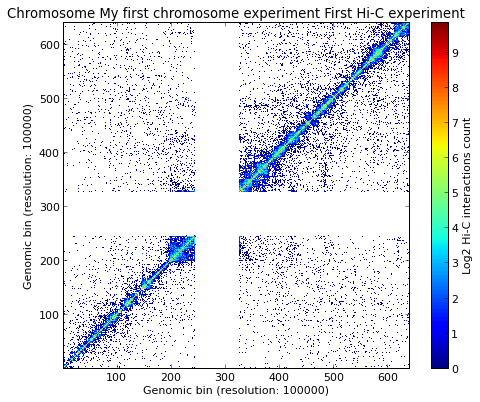
\includegraphics[max size={\textwidth}{\textheight}]{tutorial_general_files/tutorial_general_31_1.png}
    \par
    \end{center}
            \end{InvisibleVerbatim}
            
                \makebox[0.1\linewidth]{\smaller\hfill\tt\color{nbframe-out-prompt}Out\hspace{4pt}{[}13{]}:\hspace{4pt}}\\*
                \vspace{-2.55\baselineskip}\begin{InvisibleVerbatim}
                \vspace{-0.5\baselineskip}
    \begin{alltt}<matplotlib.image.AxesImage at 0x7375f50>\end{alltt}

            \end{InvisibleVerbatim}
            
        
    

    This plot shows the log2 interaction counts, resulting from the given
Hi-C experiment.

If the steps in the previous section (:ref:`run_tadbit`) have been
done and TADs habe been defined, they can
be visualized in the same kind of plot:


    % Make sure that atleast 4 lines are below the HR
    \needspace{4\baselineskip}

    
        \vspace{6pt}
        \makebox[0.1\linewidth]{\smaller\hfill\tt\color{nbframe-in-prompt}In\hspace{4pt}{[}14{]}:\hspace{4pt}}\\*
        \vspace{-2.65\baselineskip}
        \begin{ColorVerbatim}
            \vspace{-0.7\baselineskip}
            \begin{Verbatim}[commandchars=\\\{\}]
\PY{n}{my\PYZus{}chrom}\PY{o}{.}\PY{n}{visualize}\PY{p}{(}\PY{l+s}{\PYZdq{}}\PY{l+s}{First Hi\PYZhy{}C experiment}\PY{l+s}{\PYZdq{}}\PY{p}{,} \PY{n}{paint\PYZus{}tads}\PY{o}{=}\PY{n+nb+bp}{True}\PY{p}{,} \PY{n}{show}\PY{o}{=}\PY{n+nb+bp}{True}\PY{p}{)} 
\end{Verbatim}

            
                \vspace{-0.2\baselineskip}
            
        \end{ColorVerbatim}
    

    

        % If the first block is an image, minipage the image.  Else
        % request a certain amount of space for the input text.
        \needspace{4\baselineskip}
        
        

            % Add document contents.
            
                \begin{InvisibleVerbatim}
                \vspace{-0.5\baselineskip}\begin{center}
    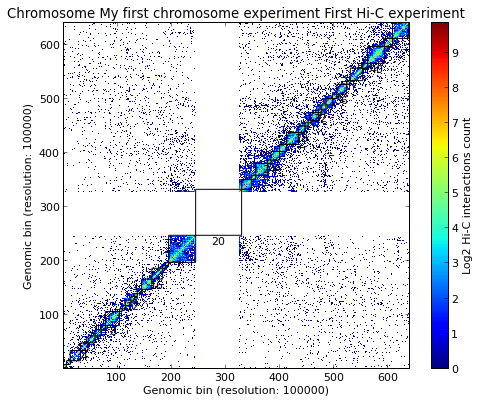
\includegraphics[max size={\textwidth}{\textheight}]{tutorial_general_files/tutorial_general_33_0.png}
    \par
    \end{center}
            \end{InvisibleVerbatim}
            
        
    

    *Note: the TAD number 19, corresponding to the centromere, and the TAD
number 18, whose size is > 3 Mb,
have been shaded*
\section{Saving and restoring data}
    In order to avoid having to calculate TAD positions each time, TADBit
allows to save and load Chromosome
objects, with all the associated experiments. To save a Chromosome
object:


    % Make sure that atleast 4 lines are below the HR
    \needspace{4\baselineskip}

    
        \vspace{6pt}
        \makebox[0.1\linewidth]{\smaller\hfill\tt\color{nbframe-in-prompt}In\hspace{4pt}{[}15{]}:\hspace{4pt}}\\*
        \vspace{-2.65\baselineskip}
        \begin{ColorVerbatim}
            \vspace{-0.7\baselineskip}
            \begin{Verbatim}[commandchars=\\\{\}]
\PY{n}{my\PYZus{}chrom}\PY{o}{.}\PY{n}{save\PYZus{}chromosome}\PY{p}{(}\PY{l+s}{\PYZdq{}}\PY{l+s}{some\PYZus{}path.tdb}\PY{l+s}{\PYZdq{}}\PY{p}{)}
\end{Verbatim}

            
                \vspace{-0.2\baselineskip}
            
        \end{ColorVerbatim}
    

    And to load it:


    % Make sure that atleast 4 lines are below the HR
    \needspace{4\baselineskip}

    
        \vspace{6pt}
        \makebox[0.1\linewidth]{\smaller\hfill\tt\color{nbframe-in-prompt}In\hspace{4pt}{[}16{]}:\hspace{4pt}}\\*
        \vspace{-2.65\baselineskip}
        \begin{ColorVerbatim}
            \vspace{-0.7\baselineskip}
            \begin{Verbatim}[commandchars=\\\{\}]
\PY{k+kn}{from} \PY{n+nn}{pytadbit} \PY{k+kn}{import} \PY{n}{load\PYZus{}chromosome}

\PY{n}{my\PYZus{}chrom} \PY{o}{=} \PY{n}{load\PYZus{}chromosome}\PY{p}{(}\PY{l+s}{\PYZdq{}}\PY{l+s}{some\PYZus{}path.tdb}\PY{l+s}{\PYZdq{}}\PY{p}{)}
\end{Verbatim}

            
                \vspace{-0.2\baselineskip}
            
        \end{ColorVerbatim}
    

    *Note: while information about TADs can be saved, in order to save
disk space, raw Hi-C data are not stored in this way but can be loaded
again for each experiment:*


    % Make sure that atleast 4 lines are below the HR
    \needspace{4\baselineskip}

    
        \vspace{6pt}
        \makebox[0.1\linewidth]{\smaller\hfill\tt\color{nbframe-in-prompt}In\hspace{4pt}{[}19{]}:\hspace{4pt}}\\*
        \vspace{-2.65\baselineskip}
        \begin{ColorVerbatim}
            \vspace{-0.7\baselineskip}
            \begin{Verbatim}[commandchars=\\\{\}]
\PY{n}{expr} \PY{o}{=} \PY{n}{my\PYZus{}chrom}\PY{o}{.}\PY{n}{experiments}\PY{p}{[}\PY{l+s}{\PYZdq{}}\PY{l+s}{First Hi\PYZhy{}C experiment}\PY{l+s}{\PYZdq{}}\PY{p}{]}

\PY{n}{expr}\PY{o}{.}\PY{n}{load\PYZus{}hic\PYZus{}data}\PY{p}{(}\PY{l+s}{\PYZdq{}}\PY{l+s}{../../scripts/sample\PYZus{}data/HIC\PYZus{}k562\PYZus{}chr19\PYZus{}chr19\PYZus{}100000\PYZus{}obs.txt}\PY{l+s}{\PYZdq{}}\PY{p}{)}
\end{Verbatim}

            
                \vspace{-0.2\baselineskip}
            
        \end{ColorVerbatim}
    


    % Make sure that atleast 4 lines are below the HR
    \needspace{4\baselineskip}

    
        \vspace{6pt}
        \makebox[0.1\linewidth]{\smaller\hfill\tt\color{nbframe-in-prompt}In\hspace{4pt}{[}{]}:\hspace{4pt}}\\*
        \vspace{-2.65\baselineskip}
        \begin{ColorVerbatim}
            \vspace{-0.7\baselineskip}
            \begin{Verbatim}[commandchars=\\\{\}]

\end{Verbatim}

            
                \vspace{-0.2\baselineskip}
            
        \end{ColorVerbatim}
    


        \renewcommand{\indexname}{Index}
        \printindex

    % End of document
    \end{document}


